% !TeX program = lualatex
% EARN — Codebase Documentation (Bangla)
\documentclass[11pt,a4paper]{article}

% ---------- Font ----------
\usepackage[a4paper,margin=2.2cm]{geometry}
\usepackage{fontspec}
\directlua{luaotfload.add_fallback(
  "bnfallback",
  {
    "Noto Serif:style=Regular;script=latn;",
    "Noto Sans Mono:style=Regular;script=latn;",
  }
)}
% Renderer=HarfBuzz + Script=Bengali are REQUIRED: LuaLaTeX's default 'node'
% renderer does not perform Indic shaping, so pre-base matras (ি ে ৈ ো ৌ) are
% not reordered before their base consonant and conjuncts do not form —
% e.g. করেন renders as করনে. Do not remove these two options.
\setmainfont{Noto Serif Bengali}[
  Renderer=HarfBuzz,
  Script=Bengali,
  RawFeature={fallback=bnfallback}
]
\setmonofont{Noto Sans Mono}[Scale=0.90]
\usepackage{underscore}

\usepackage{amsmath,amssymb}
\usepackage{booktabs,longtable,array,tabularx}
\usepackage{enumitem}
\usepackage{xcolor}
\usepackage[hidelinks]{hyperref}
\usepackage{xurl}
\usepackage{microtype}
\usepackage{fancyhdr}
\usepackage{titlesec}
\usepackage{tikz}
\usepackage{float}
\usetikzlibrary{positioning, arrows.meta, fit, backgrounds, shapes.geometric}

\definecolor{accent}{HTML}{0F4C61}
\definecolor{accent2}{HTML}{008F83}
\definecolor{softbg}{HTML}{EAF2F1}

\hypersetup{
  colorlinks=true, linkcolor=accent, urlcolor=accent,
  pdftitle={EARN Codebase Documentation},
  pdfsubject={System, database, and API documentation for the EARN study platform}
}

\titleformat{\section}{\Large\bfseries\color{accent}}{\thesection}{0.7em}{}
\titleformat{\subsection}{\large\bfseries\color{accent}}{\thesubsection}{0.6em}{}
\titleformat{\subsubsection}{\normalsize\bfseries}{\thesubsubsection}{0.5em}{}
\setlist[itemize]{leftmargin=1.6em,itemsep=0.3em,topsep=0.4em}
\setlist[enumerate]{leftmargin=1.8em,itemsep=0.35em,topsep=0.4em}
\renewcommand{\arraystretch}{1.25}
\setlength{\parindent}{0pt}
\setlength{\parskip}{0.5em}

\emergencystretch=3em
\hbadness=10000
\vbadness=10000
\hyphenpenalty=10000
\exhyphenpenalty=10000
\raggedbottom
\clubpenalty=10000
\widowpenalty=10000

\pagestyle{fancy}
\fancyhf{}
\lhead{EARN}
\rhead{Codebase Documentation}
\cfoot{\thepage}
\setlength{\headheight}{14pt}
\fancypagestyle{plain}{\fancyhf{}\cfoot{\thepage}}

\newcommand{\code}[1]{\texttt{\small #1}}
\newcommand{\file}[1]{\texttt{\small #1}}
\newcommand{\pathcode}[1]{{\small\url{#1}}}
\newcommand{\summarybox}[1]{%
  \begin{center}
  \colorbox{softbg}{\parbox{0.94\textwidth}{#1}}
  \end{center}
}

\begin{document}

% ======================================================================
\begin{titlepage}
  \centering
  \vspace*{2.0cm}
  {\Huge\bfseries\color{accent} EARN\par}
  \vspace{0.4cm}
  {\LARGE Eliciting Actionable Recommendation Feedback\par}
  \vspace{1.2cm}
  \rule{0.82\textwidth}{0.8pt}
  \vspace{1.0cm}

  {\large Codebase, database ও system architecture-এর সম্পূর্ণ টেকনিক্যাল ডকুমেন্টেশন\par}
  \vspace{0.8cm}

  \summarybox{%
    \textbf{প্রজেক্ট:} EARN একটি PhD study platform যা তিনটি ভিন্ন elicitation condition-এ
    newsletter feedback সংগ্রহ করে এবং actionability rubric দিয়ে score করে। \textbf{Stack:}
    Django REST Framework, Next.js, PostgreSQL, Docker Compose, self-hosted LLM।
  }

  \vfill
  {\large রিপোজিটরি: \texttt{/data/munna/phd\_project/earn}\par}
\end{titlepage}

\tableofcontents
\newpage

% ======================================================================
\section{ভূমিকা}

\subsection{EARN আসলে কী}

\textbf{EARN} (\textit{Eliciting Actionable Recommendation feedback from users for News
personalization}) একটি web-based research platform যা একটি PhD study চালানোর জন্য build করা
হয়েছে। Core research question হলো: একজন reader যখন একটি personalized news newsletter পড়ে
open-ended feedback দেন, কোন elicitation method reader-কে বেশি \textit{actionable} feedback
দিতে সাহায্য করে --- অর্থাৎ, এমন feedback যা একটি recommender system বাস্তবে কাজে লাগাতে পারে।

এর জন্য একটি between-subjects experiment design করা হয়েছে --- প্রতিটি participant randomly
তিনটি condition-এর একটির মধ্যে পড়েন:

\begin{enumerate}
\item \textbf{Just Ask} --- শুধু একটি neutral prompt, কোনো guidance ছাড়াই।
\item \textbf{Examples + Instructions} --- prompt-এর সাথে একটি explanation, কিছু guiding
      question এবং একটি example।
\item \textbf{Interactive Feedback Assistant} --- একটি LLM-চালিত assistant-এর সাথে ছোট
      conversation, যা reader-কে তাঁর নিজের feedback clarify করতে সাহায্য করে (কিন্তু কখনো
      তাঁর হয়ে লিখে দেয় না)।
\end{enumerate}

পরে researcher-রা প্রতিটি final feedback-কে একটি ৫-dimension actionability rubric দিয়ে score
করেন --- blind multi-rater dashboard-এর মাধ্যমে একাধিক human rater স্বাধীনভাবে score করেন
(কোনো LLM auto-rating এখন নেই)। Statistical analysis এই application-এর অংশ নয়; CSV export
থেকে R/Python-এ আলাদাভাবে করা হয়।

\summarybox{%
  এই platform feedback \textit{সংগ্রহ ও পরিমাপ} করে --- এটি কোনো live newsletter system-এ
  feedback apply করে content পরিবর্তন করে না (README-এ এটি স্পষ্টভাবে \textit{future work}
  বলে চিহ্নিত)। Newsletter-গুলো সম্পূর্ণ static/fixed stimulus, প্রতিটি participant পড়ার
  আগে থেকেই তৈরি।
}

\subsection{Stimulus: POPROX-style newsletter}

Participant-রা যে newsletter পড়েন তা real Associated Press (AP) article দিয়ে তৈরি, এবং
POPROX reference template-এর (\url{https://github.com/Mahamudul42/poprox_newsletter})
visual style follow করে (teal masthead, dark-blue section bar, thumbnail + topic-label +
serif headline + summary)। প্রতিটি newsletter-এর format fixed: \textbf{৫টি section, প্রতি
section-এ ৩টি article}। তিনটি edition বিভিন্ন topic-এ emphasis দেয় (world, US/politics,
tech/sports), যাতে feedback-এ diversity আসে। Data থাকে
\file{backend/apps/study/seed\_data/newsletters.json}-এ, \code{seed\_study} management
command দিয়ে database-এ load হয়।

\subsection{এই ডকুমেন্টের উদ্দেশ্য}

প্রজেক্ট owner হিসেবে পুরো system-টি --- architecture,
data model, প্রতিটি design decision-এর কারণ --- ভালোভাবে বোঝা দরকার। এই ডকুমেন্ট সেই
লক্ষ্যে: architecture থেকে শুরু করে প্রতিটি database table, API endpoint, frontend-এর
গুরুত্বপূর্ণ component, এবং শেষে সম্ভাব্য প্রশ্নোত্তর নিয়ে আলোচনা করা হয়েছে। প্রতিটি তথ্য
সরাসরি কোড পড়ে verify করা --- কোনো অংশ অনুমান করে লেখা হয়নি।

\newpage
% ======================================================================
\section{System Architecture}

\subsection{Tech Stack}

\begin{longtable}{@{}p{3.2cm}p{4.8cm}p{7.4cm}@{}}
\toprule
\textbf{Layer} & \textbf{Technology} & \textbf{Role} \\
\midrule
\endhead
Frontend & Next.js 16 (App Router), React 18, TypeScript, Tailwind CSS, lucide-react, Vitest
  & Participant UI \;+\; researcher dashboard \\
Backend & Django 5, Django REST Framework, SimpleJWT, drf-spectacular
  & REST API, business logic, authentication \\
Database & PostgreSQL 16 & সমস্ত persistent data \\
LLM & Self-hosted OpenAI-compatible endpoint (default model \code{openai/gpt-oss-120b})
  & Condition-3 assistant-এর জন্য \\
Container & Docker, Docker Compose & ৩-service orchestration (\S\,\ref{sec:deploy}) \\
\bottomrule
\end{longtable}

\subsection{System Diagram}

\begin{figure}[H]
\centering
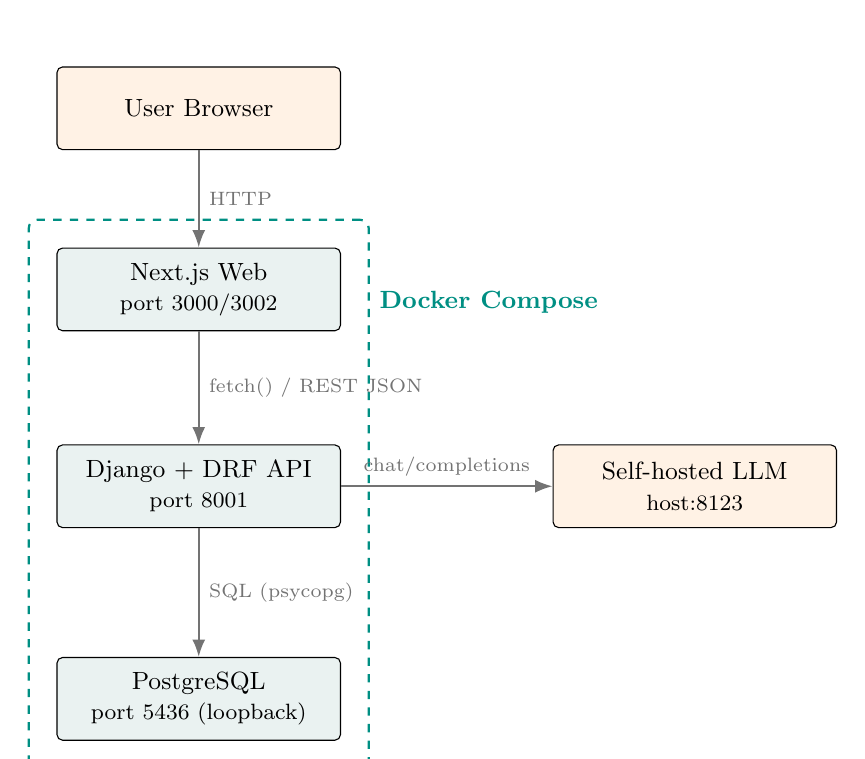
\begin{tikzpicture}[
  box/.style={draw, rounded corners=2pt, fill=softbg, minimum width=3.6cm, minimum height=1.05cm, align=center, font=\small},
  ext/.style={draw, rounded corners=2pt, fill=orange!10, minimum width=3.6cm, minimum height=1.05cm, align=center, font=\small},
  arrow/.style={-{Latex[length=2.2mm]}, thick, color=black!55}
]
  \node[ext] (browser) at (0,9.2) {User Browser};
  \node[box] (web) at (0,6.9) {Next.js Web\\\footnotesize port 3000/3002};
  \node[box] (backend) at (0,4.4) {Django + DRF API\\\footnotesize port 8001};
  \node[box] (db) at (0,1.7) {PostgreSQL\\\footnotesize port 5436 (loopback)};

  \node[ext] (llm) at (6.3,4.4) {Self-hosted LLM\\\footnotesize host:8123};

  \draw[arrow] (browser) -- (web) node[midway, right, font=\scriptsize] {HTTP};
  \draw[arrow] (web) -- (backend) node[midway, right, font=\scriptsize] {fetch() / REST JSON};
  \draw[arrow] (backend) -- (db) node[midway, right, font=\scriptsize] {SQL (psycopg)};
  \draw[arrow] (backend.east) -- (llm.west) node[midway, above, font=\scriptsize] {chat/completions};

  \begin{scope}[on background layer]
    \node[draw, dashed, accent2, thick, rounded corners=3pt, fit=(web)(backend)(db), inner sep=10pt, label={[accent2, font=\bfseries\small]above right:Docker Compose}] {};
  \end{scope}
\end{tikzpicture}
\caption{EARN-এর high-level architecture। Docker Compose তিনটি service চালায় (db, backend, web);
self-hosted LLM host machine-এর একটি আলাদা process (compose-এর বাইরে)।}
\end{figure}

\subsection{Design Rationale}

\begin{itemize}
\item \textbf{৩টি Docker service} (\code{db}, \code{backend}, \code{web}) --- \file{docker-compose.yml}-এ
  defined। কোনো আলাদা background worker নেই --- Condition-3-এর LLM call participant-এর
  নিজের request-এর মধ্যেই synchronously হয়, এবং statistical analysis এই application-এর
  বাইরে (CSV export-এর পর R/Python-এ) হয়, তাই কোনো job queue দরকার পড়েনি।
\item \textbf{\code{network\_mode: host}} backend-এ ব্যবহৃত হয়েছে যাতে container host machine-এর
  \code{127.0.0.1:8123}-এ চলা LLM-এ সরাসরি পৌঁছাতে পারে --- এই server-এ Docker-এর bridge-network
  hairpin NAT সমস্যার কারণে এটি প্রয়োজন হয়েছিল।
\item \textbf{PostgreSQL, SQLite নয়} --- production settings (\file{settings/prod.py}) নিশ্চিত
  করে যে \code{DATABASE\_URL} সবসময় PostgreSQL-এর দিকে point করে; এটি concurrent write, JSON
  field, এবং heavy statistical read-query-র জন্য বেশি উপযুক্ত।
\end{itemize}

\newpage
% ======================================================================
\section{Repository ও Code Structure}

\begin{longtable}{@{}p{6.0cm}p{9.4cm}@{}}
\toprule
\textbf{Path} & \textbf{Content} \\
\midrule
\endhead
\file{backend/apps/core/} & Health check, pagination, permission class (কোনো model নেই) \\
\file{backend/apps/users/} & JWT authentication, researcher/rater role \\
\file{backend/apps/study/} & Core app --- model, view, serializer, assignment logic, LLM
  assistant, management command \\
\file{backend/project\_backend/settings/} & \file{base.py}, \file{dev.py}, \file{prod.py}
  --- environment-driven config \\
\file{backend/system\_prompt.txt} & Condition-3 assistant-এর live system prompt (advisor-supplied,
  POPROX-specific) \\
\file{backend/tests/} & pytest test suite \\
\file{web/src/app/} & Next.js App Router page (participant \;+\; researcher) \\
\file{web/src/components/} & \file{shell/}, \file{study/}, \file{ui/} --- reusable React
  component \\
\file{web/src/lib/} & \file{api.ts} (API client), \file{auth.ts} (token), \file{types.ts}
  (TypeScript type) \\
\file{IRB/} & IRB (Institutional Review Board) protocol document \\
\file{docker-compose.yml}, \file{run.sh} & Orchestration ও operations script \\
\bottomrule
\end{longtable}

\subsection{Django App কেন তিনভাগে}

Django convention অনুযায়ী প্রতিটি ``app'' একটি self-contained responsibility বহন করে। এখানে
\code{core} (generic infrastructure), \code{users} (identity/access), এবং \code{study}
(domain logic) আলাদা রাখা হয়েছে যাতে authentication/permission code business logic থেকে আলাদা
থাকে --- এটি test করা ও পরিবর্তন করা সহজ করে।

\newpage
% ======================================================================
\section{Database Design}
\label{sec:db}

\subsection{Overview}

Study app-এ \textbf{৫টি custom model} আছে, এছাড়া Django-র built-in \code{User}/\code{Group}
table ব্যবহার করা হয়েছে researcher ও rater account-এর জন্য (আলাদা কোনো \code{Profile} model
নেই)। Migration history: \code{0001\_initial} থেকে \code{0011}-পর্যন্ত --- ১১টি migration।
প্রথম আটটি ধাপে ধাপে feature যোগ করেছে (compact survey, chat log, final draft, LLM-rating/analysis
স্কিমা, unique rating constraint); পরের তিনটি (\code{0009}--\code{0011}) সেই LLM-rating ও
analysis-সংক্রান্ত table/column বাদ দিয়েছে এবং \code{chat\_log}/\code{edition\_label}-কে
পরিষ্কার করেছে, যখন সেই feature-গুলো codebase থেকে সরিয়ে ফেলা হয়েছিল।

\begin{figure}[H]
\centering
\begin{tikzpicture}[
  ent/.style={draw, rounded corners=2pt, fill=softbg, minimum width=3.5cm, minimum height=0.95cm, align=center, font=\scriptsize, text width=3.3cm},
  usr/.style={draw, rounded corners=2pt, fill=orange!10, minimum width=3.1cm, minimum height=0.95cm, align=center, font=\scriptsize},
  rel/.style={-{Latex[length=2mm]}, color=black!55, thin}
]
  \node[ent] (news) at (0,8) {\textbf{Newsletter}\\slug, sections (JSON)};
  \node[ent] (part) at (0,5.6) {\textbf{Participant}\\public\_id (UUID), condition, status};
  \node[ent] (fb) at (-2.6,2.8) {\textbf{FeedbackResponse}\\initial\_text, final\_text,\\chat\_log (JSON), final\_draft};
  \node[ent] (sv) at (2.6,2.8) {\textbf{SurveyResponse}\\effort, express, reflect,\\understand (1--5)};
  \node[ent] (rate) at (-2.6,0.0) {\textbf{ActionabilityRating}\\৫ dimension (0--2),\\target\_level, notes};
  \node[usr] (user) at (3.4,0.0) {Django \code{User} / \code{Group}\\(manager / human\_rater)};

  \draw[rel] (news) -- (part) node[midway,right,font=\tiny]{1:N};
  \draw[rel] (part) -- (fb) node[midway,left,font=\tiny]{1:1};
  \draw[rel] (part) -- (sv) node[midway,right,font=\tiny]{1:1};
  \draw[rel] (fb) -- (rate) node[midway,left,font=\tiny]{1:N};
  \draw[rel, dashed] (user) -- (rate) node[midway,above,font=\tiny]{rater};
\end{tikzpicture}
\caption{EARN database-এর entity-relationship (ER) diagram। Dashed arrow Django \code{User}-এর
সাথে \code{ActionabilityRating.rater} relationship নির্দেশ করে (rater account delete হলে
\code{SET\_NULL})।}
\end{figure}

\subsection{Design Principles}
\begin{itemize}
\item \textbf{public\_id (UUID)} প্রতিটি \code{Participant}-এর primary key \code{id} থেকে
  আলাদা --- এটি guessable নয়, তাই URL-এ ব্যবহার করা safe, এবং এটিই participant-এর
  \textbf{completion code} হিসেবে দেখানো হয় (Prolific-compatible)।
\item \textbf{JSONField} দুই জায়গায়: \code{Newsletter.sections} (nested section/article
  structure) এবং \code{FeedbackResponse.chat\_log} (পুরো conversation)। এদের structure
  বারবার বদলায় না বলে আলাদা table না বানিয়ে JSON-এ রাখা সহজ ও যথেষ্ট।
\item \textbf{on\_delete policy সচেতনভাবে বাছাই করা}: \code{Newsletter} delete করা যাবে না যদি
  কোনো \code{Participant} সেটি ব্যবহার করে থাকে (\code{PROTECT}); কিন্তু কোনো rater account
  delete হলেও তাঁর দেওয়া rating টিকে থাকে, শুধু \code{rater} field \code{NULL} হয়ে যায়
  (\code{SET\_NULL}) --- research data কখনো হারায় না।
\item \textbf{total score store করা হয় না} --- \code{ActionabilityRating.total} একটি Python
  \code{@property} (৫টি dimension-এর sum), database-এ আলাদা column নেই, তাই কখনো
  inconsistent (stale) হতে পারে না।
\item একটি \textbf{unique constraint}: \code{(feedback, rater)} --- একজন rater একই response
  দ্বিতীয়বার rate করতে পারবেন না (\code{RatingCreateView} duplicate চেষ্টায় HTTP 409 দেয়)।
\end{itemize}

\subsection{Field Reference}

\subsubsection{Newsletter}
\begin{longtable}{@{}p{3.2cm}p{2.6cm}p{9.8cm}@{}}
\toprule
\textbf{Field} & \textbf{Type} & \textbf{Description} \\
\midrule
\endhead
\code{slug} & Slug, unique & URL-friendly identifier (যেমন \code{edition-a}) \\
\code{title} & CharField(160) & Newsletter-এর title \\
\code{sections} & JSON & \code{[\{name, articles: [\{label, headline, summary, image, url\}]\}]}
  --- fixed ৫$\times$৩ format \\
\code{is\_active} & Boolean & Inactive করলে নতুন assignment-এ ব্যবহার হবে না \\
\code{created\_at} & DateTime & auto\_now\_add \\
\bottomrule
\end{longtable}
\code{edition\_label} (যেমন ``Saturday Edition $\cdot$ June 21, 2026'') \textbf{store করা হয়
না} --- আগে একটি stored column ছিল, migration \code{0011} সেটি বাদ দিয়েছে; এখন এটি
\code{content.current\_edition\_label()} দিয়ে request-time-এ আজকের তারিখ থেকে compute হয়
(\code{SerializerMethodField}), যাতে stimulus কখনো পুরনো তারিখ দেখায় না।

\subsubsection{Participant}
\begin{longtable}{@{}p{4.6cm}p{2.6cm}p{8.2cm}@{}}
\toprule
\textbf{Field} & \textbf{Type} & \textbf{Description} \\
\midrule
\endhead
\code{public\_id} & UUID, unique & Participant-এর URL, completion code হিসেবেও ব্যবহৃত \\
\code{condition} & Integer (1/2/3) & Just Ask / Examples / Assistant \\
\code{newsletter} & FK $\to$ Newsletter (PROTECT) & কোন newsletter দেখানো হয়েছে \\
\code{recruitment\_source} & Choice & direct, movielens, prolific, other \\
\code{external\_ref} & CharField(120) & যেমন Prolific PID (\code{?ref=}) \\
\code{status} & Choice & নিচে \S\,\ref{sec:status} দেখুন \\
\code{consented\_at}, \code{completed\_at} & DateTime, nullable & \\
\code{study\_phase} & Choice & preview, pilot, main (\S\,\ref{sec:phase}) \\
\code{created\_at} & DateTime & \\
\bottomrule
\end{longtable}

\subsubsection{FeedbackResponse (Participant-এর সাথে 1:1)}
\begin{longtable}{@{}p{3.8cm}p{2.8cm}p{8.8cm}@{}}
\toprule
\textbf{Field} & \textbf{Type} & \textbf{Description} \\
\midrule
\endhead
\code{initial\_text} & Text & প্রথম যা লিখেছেন (Condition 1/2-এ final\_text-এর সমান) \\
\code{final\_text} & Text & যা submit হয়েছে (analysis-এর মূল data) \\
\code{assistant\_action} & Choice & none, suggestion, question, ok --- assistant-এর সর্বশেষ
  action \\
\code{assistant\_message} & Text & Assistant-এর সর্বশেষ message \\
\code{chat\_log} & JSON list & পুরো Condition-3 conversation:
  \code{\{role, content, action?, ts\}} \\
\code{final\_draft} & Text & LLM-consolidated draft (\S\,\ref{sec:c3}) --- \code{final\_text}
  থেকে আলাদা রাখা হয় যাতে participant কতটা edit করলেন তা measure করা যায় \\
\code{revision\_count} & PositiveInt & Condition 3-এ follow-up message-এর সংখ্যা \\
\code{time\_on\_task\_seconds} & PositiveInt, nullable & \\
\code{created\_at}, \code{updated\_at} & DateTime & \\
\bottomrule
\end{longtable}

\subsubsection{SurveyResponse (Participant-এর সাথে 1:1)}
চারটি field, প্রতিটি ১--৫ scale-এ (Likert/scale-estimation): \code{effort} (cost),
\code{express} (self-efficacy), \code{reflect} (seriousness check), \code{understand}
(perceived actionability)। প্রতিটি ভিন্ন construct measure করে (RQ3, \S\,\ref{sec:stats})।

\subsubsection{ActionabilityRating (FeedbackResponse-এর সাথে 1:N)}
\begin{longtable}{@{}p{3.9cm}p{2.6cm}p{9.1cm}@{}}
\toprule
\textbf{Field} & \textbf{Type} & \textbf{Description} \\
\midrule
\endhead
\code{rater} & FK $\to$ User, nullable & যে human rater score দিয়েছেন (rater account delete
  হলে NULL) \\
\code{target\_specificity} \newline \code{direction\_operation} \newline
  \code{collection\_allocation} \newline \code{context\_persistence} \newline
  \code{system\_feasibility} & প্রতিটি 0/1/2 & Rubric-এর ৫টি dimension
  (\S\,\ref{sec:rubric}) \\
\code{target\_level} & Choice & article, section, collection, unclear \\
\code{notes} & Text & \\
\bottomrule
\end{longtable}
\code{total} (0--10) store করা হয় না --- এটি উপরের ৫টি dimension-এর sum হিসেবে runtime-এ
compute হয়।

\subsection{Participant Status ও study\_phase}

\subsubsection{status field}
\label{sec:status}
Model-এ \textbf{৪টি} value defined: \code{created}, \code{consented}, \code{feedback},
\code{completed} (\file{apps/study/models.py}) --- একটি linear progression, \code{views.py}-র
প্রতিটি step এর মধ্যে একটিকে set করে:

\begin{center}
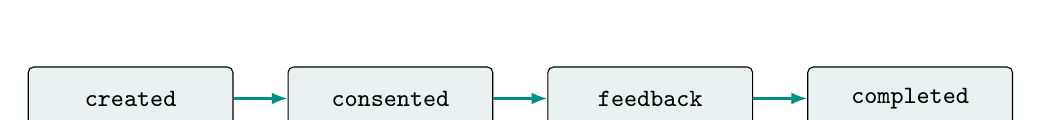
\begin{tikzpicture}
\foreach \i/\label in {0/created, 1/consented, 2/feedback, 3/completed} {
  \node[draw, rounded corners=2pt, fill=softbg, minimum width=2.6cm, minimum height=0.8cm, font=\small] (n\i) at (\i*3.3,0) {\code{\label}};
}
\foreach \i in {0,1,2} {
  \pgfmathtruncatemacro{\j}{\i+1}
  \draw[-{Latex[length=2mm]}, accent2, thick] (n\i.east) -- (n\j.west);
}
\end{tikzpicture}
\end{center}

\subsubsection{study\_phase field}
\label{sec:phase}
\begin{longtable}{@{}p{2.6cm}p{12.8cm}@{}}
\toprule
\textbf{Value} & \textbf{Meaning} \\
\midrule
\endhead
\code{preview} & \code{?condition=} বা \code{?newsletter=} দিয়ে জোর করে খোলা session
  (demo/preview)। Automatically set হয়। \\
\code{pilot} & Default --- \code{STUDY\_PHASE} environment variable set না করলে সব সাধারণ
  participant এই phase-এ পড়েন। \\
\code{main} & Real recruitment-এর আগে \code{STUDY\_PHASE=main} set করে stack restart করতে
  হয়। \\
\bottomrule
\end{longtable}
\textbf{কেন দরকার:} demo/test session যেন confirmatory analysis-এ ঢুকে না পড়ে তা নিশ্চিত
করতে। Balanced assignment (\S\,\ref{sec:assign}) এবং overview dashboard --- দুটোই phase
অনুযায়ী আলাদাভাবে count করে।

\newpage
% ======================================================================
\section{Backend: App Structure, Authentication ও Permissions}

\subsection{Settings ও Configuration}
\code{project\_backend/settings/} তিনভাগে বিভক্ত: \code{base.py} (common config),
\code{dev.py} (DEBUG=True, \code{CORS\_ALLOW\_ALL\_ORIGINS=True}), \code{prod.py} (strict
CORS/CSRF allowlist)। দুটোই PostgreSQL ব্যবহার করে --- SQLite কোথাও নেই।
\code{django-environ} library দিয়ে প্রতিটি setting environment variable থেকে আসে (root
\file{.env} file থেকে পড়া হয়) --- কোনো secret সরাসরি code-এ লেখা নেই।

মূল settings: JWT (\code{SIMPLE\_JWT}: access token ৮ ঘণ্টা, refresh token ৭ দিন), DRF
pagination (page-এ ২৫টি, \code{DefaultPagination}), \code{drf-spectacular} দিয়ে automatic
OpenAPI documentation (\code{/api/docs/})।

\subsection{Authentication: JWT}
Researcher/rater login করেন \code{/api/auth/token/}-এ username-password দিয়ে; বদলে পান
\code{access} ও \code{refresh} token (SimpleJWT)। Frontend দুটোই \code{localStorage}-এ রাখে
(\file{lib/auth.ts})। প্রতিটি API call-এ \code{Authorization: Bearer <access>} header যায়;
\code{401} পেলে \file{lib/api.ts}-এর \code{request()} function automatically \code{refresh}
token দিয়ে নতুন access token নিয়ে আবার চেষ্টা করে (একবারই, infinite loop এড়াতে
\code{retried} flag দিয়ে) --- fail হলে token মুছে login page-এ পাঠিয়ে দেয়।

Participant-দের \textbf{কোনো account লাগে না} --- \code{public\_id} (UUID)-ই তাঁদের একমাত্র
identity, যা login ছাড়াই কাজ করে (\code{permission\_classes = [AllowAny]})।

\subsection{Authorization: দুই ধরনের researcher role}
Staff user (\code{is\_staff=True}) দুইভাগে বিভক্ত, Django \code{Group} দিয়ে ---
\file{apps/users/roles.py}-এর \code{HUMAN\_RATER\_GROUP} constant-এ group-এর নাম
\code{human\_raters} defined:

\begin{longtable}{@{}p{3.4cm}p{5.6cm}p{6.4cm}@{}}
\toprule
\textbf{Permission Class} & \textbf{Condition} & \textbf{Usage} \\
\midrule
\endhead
\code{IsResearcher} & \code{is\_staff=True} (যেকোনো staff) & Response list দেখা, rating
  submit করা \\
\code{IsStudyManager} & \code{is\_staff=True} \textbf{এবং} \code{human\_raters} group-এ
  \textbf{নেই} & Overview, CSV export, rater account management \\
\bottomrule
\end{longtable}

অর্থাৎ \textbf{human rater} একটি limited role --- তাঁরা শুধু blind rating queue দেখতে
পারেন; \textbf{study manager} (মূল researcher account) সব দেখতে পারেন। Frontend-এ
\code{ResearcherShell} component \code{/api/auth/me/} call করে role জেনে navigation menu
সীমিত করে এবং rater-কে জোর করে \code{/researcher/rate}-এ পাঠিয়ে দেয় (\S\,\ref{sec:dashboard})।

\summarybox{%
  \textbf{কেন blind rating জরুরি:} human rater-রা কখনো দেখেন না কোন condition-এ feedback
  এসেছে, LLM কী score দিয়েছে, বা অন্য কোনো human rater কী score দিয়েছেন
  (\code{BlindFeedbackSerializer} শুধু \code{final\_text} পাঠায়)। এটি anchoring bias এড়ানোর
  জন্য।
}

\newpage
% ======================================================================
\section{Balanced Random Assignment}
\label{sec:assign}

প্রতিটি নতুন participant-কে (condition, newsletter)-এর একটি cell-এ বসানো হয় --- ৩টি
condition $\times$ ৩টি newsletter = ৯টি সম্ভাব্য cell। Logic আছে
\file{apps/study/assignment.py}-এর \code{choose\_cell()} function-এ:

\begin{enumerate}
\item বর্তমান \code{study\_phase}-এ (\S\,\ref{sec:phase}) প্রতিটি cell-এ এখন পর্যন্ত কতজন
  আছেন তা count করা হয়।
\item যে cell(গুলো)-তে সংখ্যা সবচেয়ে কম, তাদের মধ্যে থেকে \textbf{randomly একটি} বেছে নেওয়া
  হয় (tie ভাঙার জন্য \code{random.choice})।
\item Demo/preview link-এ (\code{?condition=3} ইত্যাদি) নির্দিষ্ট condition/newsletter জোর
  করা যায়, এবং এমন session automatically \code{study\_phase=preview} হিসেবে চিহ্নিত হয়
  (তাই এটি balance count-কে প্রভাবিত করে না)।
\end{enumerate}

এই পদ্ধতিতে enrollment বাড়ার সাথে সাথে design automatically balanced থাকে --- কোনো fixed
quota/cap ছাড়াই। \code{STUDY\_ENABLED\_CONDITIONS} environment variable দিয়ে চাইলে শুধু
condition ১ ও ২ চালানো যায় (Condition 3 optional/configurable) --- জোর-করা preview URL
তখনও যেকোনো condition-এর জন্য কাজ করবে।

\newpage
% ======================================================================
\section{Participant Flow}
\label{sec:flow}

\subsection{ধাপে ধাপে যাত্রা}

\begin{figure}[H]
\centering
\begin{tikzpicture}[
  flowstep/.style={draw, rounded corners=2pt, fill=softbg, minimum width=3.1cm, minimum height=1.1cm, align=center, font=\small},
  arrow/.style={-{Latex[length=2.2mm]}, thick, accent2}
]
  \node[flowstep] (s1) at (0,0) {১. Consent};
  \node[flowstep] (s2) at (4.2,0) {২. Newsletter +\\Feedback};
  \node[flowstep] (s3) at (8.4,0) {৩. Post-task\\Survey};
  \node[flowstep] (s4) at (12.4,0) {৪. Done\\(completion code)};
  \draw[arrow] (s1) -- (s2);
  \draw[arrow] (s2) -- (s3);
  \draw[arrow] (s3) -- (s4);
\end{tikzpicture}
\caption{Participant UI-তে চারটি step (\file{web/src/app/study/[publicId]/page.tsx})। এটি
frontend-এর client-side ``step'' state; backend-এর \code{Participant.status} আলাদা
(\S\,\ref{sec:status})।}
\end{figure}

\begin{longtable}{@{}p{1.0cm}p{4.6cm}p{9.8cm}@{}}
\toprule
\textbf{Step} & \textbf{API Call} & \textbf{যা ঘটে} \\
\midrule
\endhead
0 & \url{POST /api/session/start/} & \code{BeginButton} URL-এর query parameter (\code{source},
  \code{ref}, \code{condition}, \code{newsletter}) পড়ে এই call করে। Backend
  \code{choose\_cell()} দিয়ে (condition, newsletter) ঠিক করে নতুন \code{Participant} তৈরি
  করে, তারপর \code{/study/<public\_id>}-এ redirect করে। \\
1 & \url{POST /api/session/<public_id>/consent/} & Consent text দেখানোর পর ``I agree'' চাপলে
  \code{consented\_at} ও \code{status=consented} set হয় (idempotent)। \\
2a & \url{POST /api/session/<public_id>/feedback/initial/} & Newsletter ও feedback-form একই
  page-এ (POPROX-এর নিজস্ব end-of-newsletter feedback block-এর মতো)। Condition 1/2-এ এখানেই
  \code{final\_text} set হয়ে যায়; Condition 3-এ প্রথম assistant turn শুরু হয়। \\
2b & \url{POST .../feedback/chat/}, \url{.../feedback/final-draft/} & শুধু Condition 3 ---
  \S\,\ref{sec:c3} দেখুন। \\
2c & \url{POST /api/session/<public_id>/feedback/final/} & \code{final\_text},
  \code{time\_on\_task\_seconds}, \code{revision\_count} save হয়। \\
3 & \url{POST /api/session/<public_id>/survey/} & ৪-item survey submit; \code{status=completed},
  \code{completed\_at} set হয়। \\
4 & --- & Done screen-এ \code{public\_id} completion code হিসেবে দেখানো হয় (Prolific-compatible)। \\
\bottomrule
\end{longtable}

\newpage
% ======================================================================
\section{তিনটি Feedback-Elicitation Condition}

Copy (participant-facing text) backend-এ রাখা হয়েছে (\file{apps/study/content.py}),
frontend-এ নয় --- যাতে wording pilot-এর পর code না ছুঁয়ে ঠিক করা যায়। সব condition-এ একই
core prompt: \textit{``How would you like this newsletter to work better for you?''} ---
ইচ্ছাকৃতভাবে neutral, শুধু topic-centric নয়।

\begin{longtable}{@{}p{2.4cm}p{6.4cm}p{7.0cm}@{}}
\toprule
\textbf{Condition} & \textbf{Participant যা দেখেন} & \textbf{Design rationale} \\
\midrule
\endhead
1. Just Ask & শুধু core prompt \;$+$\; একটি short explanation, কোনো example/support নেই &
  Baseline --- minimal guidance-এ মানুষ naturally কী লেখেন তা measure করা (RQ1) \\
2. Examples + Instructions & Prompt \;$+\;$ একটি neutral instruction \;$+\;$ multiple
  dimension-এর guiding question (topic, tone, scope, source, length ইত্যাদি) \;$+\;$ একটি
  example & Static support কতটা সাহায্য করে তা measure করা, কিন্তু কোনো নির্দিষ্ট topic/opinion-এর
  দিকে না ঠেলে \\
3. Interactive Assistant & Prompt \;$+\;$ একটি LLM assistant-এর সাথে ছোট conversation যা
  clarifying question/suggestion দেয়, কখনো লিখে দেয় না & Interactive support static-এর চেয়ে
  বেশি সাহায্য করে কিনা তা measure করা (\S\,\ref{sec:c3}) \\
\bottomrule
\end{longtable}

Condition 2-এর example/guidance ইচ্ছাকৃতভাবে multi-dimensional --- শুধু ``topic'' নয়, বরং
tone, locality, person/organization, depth, source type, section-mix, recency, length,
diversity, ও context/background --- যাতে participant-রা কোনো নির্দিষ্ট দিকে না ঠেলে যান।

\newpage
% ======================================================================
\section{Condition 3: Interactive Feedback Assistant}
\label{sec:c3}

এটি codebase-এর সবচেয়ে জটিল অংশ (\file{apps/study/assistant.py}, ৩৫১ লাইন)।

\subsection{Strict Rules}
System prompt-এ স্পষ্টভাবে লেখা --- assistant কখনো:
\begin{itemize}
\item Participant-এর কথা \textbf{rewrite/polish} করবে না;
\item নতুন কোনো preference, topic, entity, বা source \textbf{invent/suggest} করবে না;
\item কোনো নির্দিষ্ট topic/opinion/source-এর দিকে participant-কে \textbf{lead} করবে না;
\item Sensitive/personal information পেলে neutrally সতর্ক করবে, কোনো judgement ছাড়া।
\end{itemize}
এর বদলে সে শুধু ১--২টি short, concrete suggestion দেয় বা একটি clarifying question করে ---
এবং feedback ইতিমধ্যে actionable হলে তা paraphrase করে confirm করে।

\subsection{System Prompt কোথায় থাকে}
Live prompt থাকে \file{backend/system\_prompt.txt}-এ (advisor-supplied, POPROX-specific), যা
git-tracked এবং Docker image-এ \textbf{bake} করা থাকে --- অর্থাৎ এই file পরিবর্তন করলে backend
image পুনরায় build করতে হয় (\code{docker compose up -d --build backend})। এই file সবসময়
present থাকে বলে কোনো embedded fallback prompt নেই --- file missing বা খালি হলে
\code{\_load\_system\_prompt()} সরাসরি error raise করে, যাতে কখনো ভিন্ন/stale prompt নিঃশব্দে
চালু না হয়ে যায়।

\subsection{Conversation Flow}

\begin{figure}[H]
\centering
\begin{tikzpicture}[
  n/.style={draw, rounded corners=2pt, fill=softbg, minimum width=3.3cm, minimum height=1.0cm, align=center, font=\small},
  d/.style={draw, diamond, aspect=2.4, fill=orange!10, minimum width=3.0cm, align=center, font=\scriptsize},
  arrow/.style={-{Latex[length=2mm]}, thick, black!55}
]
  \node[n] (init) at (0,7) {Participant প্রাথমিক\\feedback লেখেন};
  \node[d] (act) at (0,5) {Assistant-এর\\action?};
  \node[n] (q) at (-4.3,3) {question / suggestion\\(chat চলতে থাকে)};
  \node[n] (ok) at (4.3,3) {ok\\(actionable)};
  \node[n] (reply) at (-4.3,1) {Participant উত্তর দেন\\(feedback/chat/)};
  \node[n] (draft) at (4.3,1) {Consolidate draft তৈরি\\(feedback/final-draft/)};
  \node[n] (edit) at (0,-1.1) {Participant draft\\দেখেন \& edit করেন};
  \node[n] (submit) at (0,-3.1) {Final submit\\(feedback/final/)};

  \draw[arrow] (init) -- (act);
  \draw[arrow] (act) -- (q);
  \draw[arrow] (act) -- (ok);
  \draw[arrow] (q) -- (reply);
  \draw[arrow] (reply.south) to[out=-90,in=180] (act.west);
  \draw[arrow] (ok) -- (draft);
  \draw[arrow] (draft) -- (edit);
  \draw[arrow] (edit) -- (submit);
  \draw[arrow, dashed] (q.south) .. controls (-4.3,-1.6) and (-1.5,-1.6) .. (edit.west) node[midway, below, font=\tiny]{``I'm done''};
\end{tikzpicture}
\caption{Condition-3 conversation loop। Participant চাইলে যেকোনো সময় ``I'm done'' চেপে সরাসরি
review-panel-এ যেতে পারেন (dashed arrow)।}
\end{figure}

প্রতিটি turn-এ assistant \textbf{শুধুমাত্র একটি JSON object} return করে:
\begin{center}
\small\ttfamily \{"action": "suggestion" $\vert$ "question" $\vert$ "ok", "message": "..."\}
\end{center}
\code{CONVERSATION\_ADDENDUM} মূল prompt-এর সাথে জোড়া লাগে যাতে এটি multi-turn
conversation-এ মানিয়ে নেয় (একই question দুবার না করা, একটি turn-এ সর্বোচ্চ একটি question)।

\subsection{Newsletter Grounding (read-only context)}
Assistant naturally শুধু conversation দেখে --- তাই ``প্রথম গল্পটা'' বা ``যুদ্ধের কভারেজ''
বললে বুঝতে পারবে না তা কী বোঝাচ্ছে। এই সমস্যা সমাধানে \code{render\_newsletter\_context()}
participant যে নির্দিষ্ট newsletter পড়েছেন তা system prompt-এর সাথে জুড়ে দেয় --- কিন্তু
কঠোরভাবে ``শুধু reference, suggestion-এর উৎস নয়'' হিসেবে চিহ্নিত করে একটি anti-leading
guardrail সহ, যাতে assistant newsletter থেকে এমন কিছু suggest না করে যা participant নিজে
তোলেননি (এটি study-কে bias করত)।

\subsection{Local-only Model Client --- কোনো Fallback নেই}
\code{assistant.py} একটি self-hosted, OpenAI-compatible endpoint-এ (\code{LOCAL\_LLM\_BASE\_URL},
default model \code{openai/gpt-oss-120b}) call করে --- \textbf{বাইরের কোনো provider import
করা নেই, এবং কোনো rule-based fallback-ও নেই।} Call fail হলে (endpoint unreachable, timeout,
বা parse করতে না পারা JSON) \code{AssistantUnavailable} exception raise হয়, যা view-তে
HTTP \code{503} হিসেবে ফিরে যায়। Frontend তখন participant-কে জানায় assistant এই মুহূর্তে
পাওয়া যাচ্ছে না, এবং participant ততক্ষণে যা লিখেছেন তা নিয়েই submit করতে পারেন --- কোনো
canned/deterministic reply দিয়ে চুপচাপ চালিয়ে দেওয়া হয় না।

\summarybox{%
  \textbf{কেন external LLM provider ব্যবহার করা হয়নি:} participant-এর raw feedback (কখনো
  sensitive information সহ) third-party API-তে না পাঠাতে সচেতনভাবে শুধুমাত্র self-hosted
  local model ব্যবহার করা হয়েছে --- এটি IRB-approved privacy protection-এর সাথে consistent।
  Fail হলে data বাইরে না পাঠিয়ে সরাসরি \code{503} দেওয়া হয়, কোনো বিকল্প generated text দিয়ে
  ভরাট করা হয় না।
}

\subsection{Final Consolidation (final\_draft বনাম final\_text)}
যখন assistant \code{"ok"} বলে বা participant ``I'm done'' চাপেন, frontend
\url{POST .../feedback/final-draft/} call করে। Backend-এর \code{compose\_final\_feedback()}
পুরো conversation-কে একটি single, first-person statement-এ consolidate করে --- এটি একই
\code{SYSTEM\_PROMPT}-এর উপর ভিত্তি করে চলে, শুধু \code{FINALIZE\_PROMPT} output-format ও
task পাল্টে দেয় (JSON turn-reply-এর বদলে একটি plain paragraph), বাকি সব rule (neutrality,
কিছু invent না করা) অক্ষুণ্ণ থাকে। এই draft \code{final\_draft}-এ save হয় এবং participant-কে
editable textbox-এ দেখানো হয়।

\textbf{Participant এই draft স্বাধীনভাবে edit করতে পারেন} --- যা শেষ পর্যন্ত submit হয় তা
\code{final\_text}-এ যায়। \code{final\_draft} ও \code{final\_text} ইচ্ছাকৃতভাবে আলাদা column-এ
রাখা হয়েছে, যাতে researcher-রা measure করতে পারেন participant-রা LLM-এর তৈরি draft কতটা
faithfully রাখলেন বা কতটা পরিবর্তন করলেন (faithfulness/edit-distance analysis)।

\textbf{Consolidation বনাম rewriting-এর পার্থক্য:} Strict rules বলে assistant কখনো
participant-এর কথা rewrite করবে না --- তাহলে consolidation step কি rule ভাঙছে? না, কারণ এটি
structurally আলাদা একটি step: এটি conversation \textit{চলাকালীন} ঘটে না (তাই participant-কে
influence করতে পারে না), শুধুমাত্র তাঁর নিজের কথাগুলো একত্র/সাজিয়ে দেখায়, এবং সবচেয়ে
গুরুত্বপূর্ণ --- participant এটি \textbf{সবসময় দেখেন, edit করতে পারেন, এবং explicitly
confirm না করলে submit হয় না}।

\subsection{Actionability Rubric}
\label{sec:rubric}
Human rater-রা \pathcode{/researcher/rate}-এ প্রতিটি final feedback একই ৫-dimension rubric-এ
score করেন (\S\,\ref{sec:dashboard})। আগে একটি LLM auto-rater (একই rubric-এ
\code{final\_text} স্বয়ংক্রিয়ভাবে score করত) codebase-এ ছিল, কিন্তু সেটি এবং সংশ্লিষ্ট
background job queue \& statistics pipeline সরিয়ে ফেলা হয়েছে --- এখন rating সম্পূর্ণভাবে
human, এবং analysis CSV export-এর পর externally (R/Python-এ) হয়।

\begin{longtable}{@{}p{3.9cm}p{11.3cm}@{}}
\toprule
\textbf{Dimension (0/1/2)} & \textbf{কী measure করে} \\
\midrule
\endhead
\code{target\_specificity} & একটি concrete target বলা হয়েছে কি (topic, entity, event,
  geography, source, section) \\
\code{direction\_operation} & স্পষ্ট operation বলা হয়েছে কি (include, exclude, prioritize,
  diversify, reduce, reorder) \\
\code{collection\_allocation} & সামগ্রিক mix, variety, repetition নিয়ে বলা হয়েছে কি \\
\code{context\_persistence} & কখন applicable, কতদিন persist করে, কোন exception আছে তা বলা
  হয়েছে কি \\
\code{system\_feasibility} & POPROX-এর available AP article-pool ও supported operation দিয়ে
  satisfy করা যায় কিনা \\
\bottomrule
\end{longtable}
প্রতিটি dimension 0 (absent/unusable), 1 (partial/implied), বা 2 (clear ও directly usable)
--- total 0--10। সাথে \code{target\_level} (article, section, collection, unclear) ও একটি
short \code{notes}।

\newpage
% ======================================================================
\section{Researcher Dashboard}
\label{sec:dashboard}

সব page \code{/researcher/*}-এর নিচে, \code{ResearcherShell} component দিয়ে wrap করা
(JWT-guard, role-based navigation, CSV export button)।

\begin{longtable}{@{}p{3.0cm}p{2.2cm}p{10.8cm}@{}}
\toprule
\textbf{Page} & \textbf{Access} & \textbf{কী করে} \\
\midrule
\endhead
\pathcode{/researcher} (Overview) & Manager & Enrollment count (total, completed,
  final-response, rated), condition-wise table, ও (condition $\times$ newsletter)
  balance-grid \\
\pathcode{/researcher/rate} (Blind rating) & Rater \;+\; Manager & এক-এক করে blind queue
  থেকে response দেখায় (শুধু \code{final\_text}); ৫-dimension 0, 1, 2 button,
  \code{target\_level} chip, notes, Save/Skip। Save-এর পর queue থেকে সরে যায়। \\
\pathcode{/researcher/raters} (Raters) & Manager & নতুন rater তৈরি (username, email,
  temporary password, generator সহ), rating-count, last-login, active-status table, password
  reset বা deactivate; নতুন credential একবারই দেখানো হয় \\
\bottomrule
\end{longtable}

\summarybox{%
  \textbf{একাধিক human rater management:} মূল researcher account (study manager)
  \pathcode{/researcher/raters} থেকে যতজন ইচ্ছা human rater তৈরি করতে পারেন --- প্রতিটি
  rater-এর নিজস্ব login, কখনো account share করা উচিত না (কারণ প্রতিটি score সেই
  rater-identity-র সাথে জড়িয়ে থাকে, যা পরে externally inter-rater reliability হিসাব করতে
  কাজে লাগে)।
}

\newpage
% ======================================================================
\section{Statistical Analysis}
\label{sec:stats}

আগে \file{apps/study/statistics.py}-তে একটি in-app RQ1--RQ3 statistics pipeline ছিল (OLS
regression with HC3 robust SE, Holm-corrected planned contrast, Hedges' g effect size,
ordinal logistic regression, human$\leftrightarrow$LLM agreement/ICC/kappa ইত্যাদি) --- এই
ফাইল ও এর সাথে জড়িত dashboard/API সম্পূর্ণভাবে সরিয়ে ফেলা হয়েছে।

\textbf{বর্তমান অবস্থা:} statistical analysis এই application-এর অংশ \textbf{নয়}।
\pathcode{/api/research/export.csv} থেকে (condition, newsletter, phase, initial/final/draft
text, survey score, human-rating mean, সম্পূর্ণ \code{chat\_log} সহ) সম্পূর্ণ CSV নামিয়ে
analysis externally R/Python-এ করা হয়।

\newpage
% ======================================================================
\section{API Reference}

সব endpoint \code{/api/} দিয়ে শুরু। Interactive documentation: \url{/api/docs/} (Swagger)
ও \url{/api/redoc/} (drf-spectacular দিয়ে automatically generated, তাই code-এর সাথে সবসময়
sync থাকে)।

\subsubsection*{Participant (public, কোনো login লাগে না)}
\begin{longtable}{@{}p{1.7cm}p{6.9cm}p{7.4cm}@{}}
\toprule
\textbf{Method} & \textbf{Path} & \textbf{Description} \\
\midrule
\endhead
POST & \url{/api/session/start/} & নতুন session (balanced/forced assignment) \\
GET & \url{/api/session/<public_id>/} & Session \;+\; newsletter \;+\; condition-copy \\
POST & \url{/api/session/<public_id>/consent/} & Consent record \\
POST & \url{/api/session/<public_id>/feedback/initial/} & প্রাথমিক feedback (\;+\; C3 হলে
  প্রথম assistant turn) \\
POST & \url{/api/session/<public_id>/feedback/chat/} & C3: পরবর্তী conversation-turn \\
POST & \url{/api/session/<public_id>/feedback/final-draft/} & C3: consolidated draft তৈরি \\
POST & \url{/api/session/<public_id>/feedback/final/} & Final feedback submit \\
POST & \url{/api/session/<public_id>/survey/} & Post-task survey submit; \code{status=completed} \\
\bottomrule
\end{longtable}

\subsubsection*{Authentication}
\begin{longtable}{@{}p{1.7cm}p{6.9cm}p{7.4cm}@{}}
\toprule
\textbf{Method} & \textbf{Path} & \textbf{Description} \\
\midrule
\endhead
POST & \url{/api/auth/token/} & Login (JWT access \;+\; refresh) \\
POST & \url{/api/auth/token/refresh/} & Access token refresh \\
GET & \url{/api/auth/me/} & বর্তমান user-এর তথ্য ও role \\
GET/POST & \url{/api/auth/raters/} & Rater list ও তৈরি (manager only) \\
PATCH & \url{/api/auth/raters/<id>/} & Rater update, deactivate, বা password reset (manager only) \\
\bottomrule
\end{longtable}

\subsubsection*{Researcher Dashboard}
\begin{longtable}{@{}p{1.7cm}p{6.9cm}p{7.4cm}@{}}
\toprule
\textbf{Method} & \textbf{Path} & \textbf{Description} \\
\midrule
\endhead
GET & \url{/api/research/overview/} & Enrollment summary (manager) \\
GET & \url{/api/research/responses/} & Response list; \code{?condition=}, \code{?newsletter=},
  \code{?phase=}, \code{?unrated=1} \\
GET & \url{/api/research/responses/<id>/} & একক response detail (manager) \\
POST & \url{/api/research/responses/<id>/ratings/} & নতুন human rating submit; duplicate হলে
  \code{409} \\
GET & \url{/api/research/export.csv} & সম্পূর্ণ CSV export (manager) \\
\bottomrule
\end{longtable}

\textbf{অন্যান্য:} \url{/api/health/} (health check, AllowAny), \url{/admin/} (Django admin),
\url{/api/schema/} (OpenAPI JSON schema)।

\newpage
% ======================================================================
\section{Frontend Architecture}

\subsection{Folder Organization}
Next.js \textbf{App Router} ব্যবহার করা হয়েছে (\file{web/src/app/}) --- প্রতিটি folder একটি
route।

\begin{longtable}{@{}p{5.2cm}p{10.2cm}@{}}
\toprule
\textbf{Path} & \textbf{কী} \\
\midrule
\endhead
\pathcode{app/page.tsx} & Homepage --- short description \;+\; ``Begin the study'' button \\
\pathcode{app/study/[publicId]/page.tsx} & মূল participant wizard (consent, তারপর
  newsletter+feedback, তারপর survey, তারপর done) \\
\pathcode{app/researcher/*} & Login \;+\; ৩টি dashboard page: overview, rate, raters
  (\S\,\ref{sec:dashboard}) \\
\pathcode{components/shell/} & \code{StudyHeader}, \code{ResearcherShell} (navigation \;+\;
  auth-guard) \\
\pathcode{components/study/} & \code{BeginButton}, \code{NewsletterView}, \code{FeedbackStep},
  \code{SurveyStep} \\
\pathcode{components/ui/} & \code{Button}, \code{Card}, \code{Badge}, \code{Likert},
  \code{Spinner}, \code{Textarea} --- ছোট, reusable UI primitive \\
\pathcode{lib/api.ts} & একক typed fetch-client; JWT auto-refresh logic এখানেই \\
\pathcode{lib/auth.ts} & \code{localStorage}-এ token রাখা ও পড়া \\
\pathcode{lib/types.ts} & Backend serializer-এর সাথে হুবহু মিলিয়ে রাখা TypeScript interface \\
\bottomrule
\end{longtable}

\subsection{Key Component: NewsletterView}
\code{NewsletterView} POPROX-এর visual language হুবহু code করে reproduce করে --- teal
(\code{\#008F83}) masthead, navy (\code{\#003C5E}) section-bar, প্রতিটি article-এর thumbnail,
label, serif headline, summary। Image load fail হলে (\code{onError}) একটি label-সহ
placeholder দেখায়, যাতে broken image participant-এর experience নষ্ট না করে।

\subsection{Key Component: FeedbackStep}
এই component-টি (৩৬৮ লাইন) condition ১, ২, ৩ --- তিনটিরই UI single file-এ ধারণ করে, একটি
ছোট state machine দিয়ে:

\begin{itemize}
\item \code{phase: "writing" | "chat"} --- প্রথমে সবাই লেখেন; শুধু Condition 3-এ
  \code{"chat"} phase চালু হয় (যদি প্রথম assistant-action \code{"none"} না হয়)।
\item \code{finalDirtyRef} (একটি \code{useRef}) --- participant একবার draft হাতে edit
  করলে, নতুন chat-turn-এ আর automatically draft refresh/overwrite হয় না --- তাঁদের edit
  respect করা হয়।
\item \textbf{Optimistic UI} --- \code{handleSend()}-এ user-এর message তাৎক্ষণিকভাবে chat-এ
  দেখানো হয় (server response-এর জন্য wait না করে); fail হলে rollback করে draft ফিরিয়ে দেয়।
\item \code{seconds()} helper \code{time\_on\_task\_seconds} measure করে।
\item Enter-key chat-এ message পাঠায় (Shift+Enter নতুন line) --- চ্যাট-অ্যাপের প্রচলিত UX
  pattern।
\end{itemize}

\subsection{API Client: JWT Auto-refresh}
\file{lib/api.ts}-এর \code{request()} function প্রতিটি call-এ ৪০১ পেলে (এবং আগে retry না করা
থাকলে) automatically \code{refreshAccessToken()} call করে, নতুন access token দিয়ে একবার আবার
চেষ্টা করে। একাধিক parallel request একই সময়ে ৪০১ পেলে, একটিমাত্র refresh-request share হয়
(\code{refreshRequest} promise variable দিয়ে)।

\newpage
% ======================================================================
\section{Deployment ও Operations}
\label{sec:deploy}

\subsection{Docker Compose Services}
\begin{longtable}{@{}p{2.6cm}p{6.4cm}p{6.8cm}@{}}
\toprule
\textbf{Service} & \textbf{Image/Command} & \textbf{Note} \\
\midrule
\endhead
\code{db} & \code{postgres:16} & Loopback-only port (\code{127.0.0.1:5436}),
  \code{pg\_isready} healthcheck \\
\code{backend} & \file{backend/Dockerfile} (Django, Gunicorn) & \code{network\_mode: host};
  startup-এ migrate + seed\_study automatically চলে \\
\code{web} & \file{web/Dockerfile} (multi-stage: builder + runner) &
  \code{NEXT\_PUBLIC\_API\_BASE\_URL} \textbf{build-time-এ} bake হয় (Next.js-এর নিয়ম) \\
\bottomrule
\end{longtable}

\summarybox{%
  \textbf{গুরুত্বপূর্ণ:} backend ও web দুটোরই Dockerfile source code image-এ copy করে ---
  কোনো volume mount নেই। তাই code পরিবর্তনের পর শুধু container restart করলে হবে না; image
  পুনরায় build করতে হয়: \code{docker compose up -d --build backend} (বা \code{web})। এটি না
  করলে stale code চলতেই থাকবে।
}

\subsection{run.sh --- Convenience Wrapper Script}
\begin{longtable}{@{}p{3.6cm}p{12.4cm}@{}}
\toprule
\textbf{Command} & \textbf{কাজ} \\
\midrule
\endhead
\code{./run.sh up} & Build \;+\; সম্পূর্ণ stack background-এ চালু \\
\code{./run.sh down} / \code{restart} & বন্ধ/পুনরায় চালু (database volume অক্ষত থাকে) \\
\code{./run.sh reset} & \textbf{Database volume মুছে} নতুন করে শুরু (re-seed) \\
\code{./run.sh rebuild} & শূন্য থেকে image পুনর্নির্মাণ \\
\code{./run.sh logs [svc]}, \code{ps} & Log/status দেখা \\
\code{./run.sh seed} / \code{migrate} / \code{superuser} & Seed/migrate/superuser \\
\code{./run.sh manage <args>} / \code{shell} & Backend container-এ \code{manage.py} বা shell \\
\bottomrule
\end{longtable}

\subsection{Environment Variables}
\begin{longtable}{@{}p{5.2cm}p{2.0cm}p{9.0cm}@{}}
\toprule
\textbf{Name} & \textbf{Where} & \textbf{কাজ} \\
\midrule
\endhead
\code{DATABASE\_URL} & backend & PostgreSQL DSN \\
\code{DJANGO\_SECRET\_KEY}, \newline \code{DJANGO\_DEBUG}, \newline
  \code{DJANGO\_ALLOWED\_HOSTS} & backend & Core Django settings \\
\code{CORS\_ALLOWED\_ORIGINS}, \newline \code{CORS\_ALLOW\_ALL\_ORIGINS}, \newline
  \code{CSRF\_TRUSTED\_ORIGINS} & backend & Browser-security \\
\code{RESEARCHER\_USERNAME}, \newline \code{RESEARCHER\_PASSWORD} & backend & Seeded dashboard
  login \\
\code{LOCAL\_LLM\_BASE\_URL}, \newline \code{LOCAL\_LLM\_MODEL}, \newline
  \code{LOCAL\_LLM\_API\_KEY}, \newline \code{LOCAL\_LLM\_TIMEOUT\_SECONDS} & backend &
  Condition-3 assistant (\S\,\ref{sec:c3}) \\
\code{STUDY\_ENABLED\_CONDITIONS} & backend & Balanced assignment-এ active condition
  (\S\,\ref{sec:assign}) \\
\code{STUDY\_PHASE} & backend & \code{pilot} (default) বা \code{main} (\S\,\ref{sec:phase}) \\
\code{BACKEND\_PORT}, \newline \code{WEB\_PORT}, \code{DB\_PORT} & compose & Port mapping \\
\code{NEXT\_PUBLIC\_API\_BASE\_URL} & web (build-time) & Browser থেকে backend-এর URL \\
\code{POSTGRES\_DB}, \newline \code{POSTGRES\_USER}, \newline \code{POSTGRES\_PASSWORD} &
  compose & Database credential \\
\bottomrule
\end{longtable}

\subsection{Port Map}
Default: web \code{3000}, backend \code{8001}, DB \code{5436} (loopback-only)। \textbf{এই
server-এ} (অন্যান্য project 3000/3001 ব্যবহার করায়) \code{.env}-এ \code{WEB\_PORT=3002} set
করা --- তাই এই server-এ participant site \url{http://localhost:3002}। Backend container
\code{network\_mode: host} ব্যবহার করে যাতে host-এর \code{127.0.0.1:8123}-এ চলা local LLM-এ
পৌঁছাতে পারে। Remote থেকে demo দেখাতে হলে দুটো port-ই SSH দিয়ে forward করতে হয়।

\newpage
% ======================================================================
\section{Testing ও Quality}

\begin{itemize}
\item \textbf{Backend}: \code{pytest} (\file{backend/tests/}) --- auth, assistant logic,
  balanced assignment, full flow, permission cover করে। Production image-এ \code{pytest}
  থাকে না (light রাখতে); run করতে container-এ \code{pip install pytest pytest-django} লাগে।
\item \textbf{Frontend}: \code{npm run test} (Vitest), \code{npm run lint} (ESLint,
  \code{next/core-web-vitals}), \code{npm run build} (production build \;+\; TypeScript
  type-check)।
\end{itemize}

\newpage
% ======================================================================
\section{Security ও Privacy Considerations}
\label{sec:security}

\begin{itemize}
\item \textbf{কোনো PII সংগ্রহের design নেই} --- consent-text-এ স্পষ্টভাবে request করা হয়
  নাম, ঠিকানা, ইমেইল, ফোন না লিখতে; assistant sensitive information দেখলে neutrally সতর্ক
  করে (\S\,\ref{sec:c3})।
\item \textbf{Data তৃতীয়-পক্ষের কাছে যায় না} --- LLM call শুধু self-hosted local
  endpoint-এ যায়, কোনো বাইরের API (OpenAI, Google ইত্যাদি) নেই।
\item \textbf{JWT স্বল্পস্থায়ী} --- access token ৮ ঘণ্টা, refresh ৭ দিন; সব researcher-endpoint
  \code{IsAuthenticated} (default) $+$ \code{IsResearcher} বা \code{IsStudyManager} দিয়ে
  সুরক্ষিত।
\item \textbf{CORS/CSRF} স্পষ্টভাবে allowlist-ভিত্তিক production-এ (\code{CORS\_ALLOW\_ALL\_ORIGINS}
  default বন্ধ)।
\item \textbf{Rating overwrite করা যায় না} --- একজন rater একটি response একবারই score করতে
  পারেন (\code{unique(feedback, rater)}); ভুল score ঠিক করতে database-level access লাগে,
  accidental double-submit থেকে data protect থাকে (\S\,\ref{sec:db})।
\item \textbf{Secret environment variable-এ} --- \file{.env} \code{.gitignore}-এ (repo-তে
  শুধু \file{.env.example}); default password production-এ অবশ্যই পাল্টাতে হবে।
\end{itemize}

\newpage
% ======================================================================
\section{সম্ভাব্য প্রশ্ন ও উত্তর}

\begin{enumerate}[leftmargin=*, label=\textbf{প্রশ্ন \arabic*.}]

\item \textbf{ব্যাকএন্ডে Django + DRF কেন বেছে নেওয়া হলো, অন্য কিছু না?}\\
উত্তর: Research study-তে দ্রুত ও নির্ভরযোগ্য data-modeling জরুরি --- Django-র ORM, built-in
admin panel (data দ্রুত inspect করার জন্য), migration system, এবং DRF-এর serializer/permission
framework এই ধরনের CRUD-heavy, permission-sensitive application-এর জন্য proven ও দ্রুত
development দেয়।

\item \textbf{কেন PostgreSQL, আর JSONField কেন দরকার হলো?}\\
উত্তর: \code{chat\_log} ও \code{sections}-এর structure nested ও variable (প্রতিটি
conversation-এ ভিন্ন সংখ্যক turn) --- এর জন্য প্রতিটি turn-এর জন্য আলাদা table বানানো
unnecessary complexity যোগ করত। PostgreSQL-এর native JSONField এখানে উপযুক্ত।

\item \textbf{Participant-দের কীভাবে identify করা হয়? তাদের কি account লাগে?}\\
উত্তর: না। প্রতিটি session-এর একটি random UUID (\code{public\_id}) --- এটিই তাঁদের URL এবং
সবশেষে completion code। কোনো password/login লাগে না, যা research-এ participation friction
কমায়।

\item \textbf{Condition 3-এ assistant কীভাবে participant-এর কথা বদলে দেওয়া থেকে বিরত থাকে?}\\
উত্তর: তিনটি স্তরে --- (ক) system prompt-এ স্পষ্ট strict rules (rewrite, invent, lead করবে
না); (খ) structurally chat ও final consolidation আলাদা step; (গ) participant সবসময় final
text নিজে দেখেন, edit করতে পারেন, এবং explicitly confirm না করলে কিছুই submit হয় না।

\item \textbf{Local LLM যদি fail বা down হয়, তখন কী হয়?}\\
উত্তর: কোনো fallback নেই --- backend \code{AssistantUnavailable} raise করে, যা HTTP
\code{503} হিসেবে ফিরে যায়। Frontend participant-কে জানায় assistant এই মুহূর্তে পাওয়া
যাচ্ছে না; participant ততক্ষণে যা লিখেছেন তা নিয়েই submit করতে পারেন।

\item \textbf{বাইরের LLM provider (OpenAI, Gemini ইত্যাদি) কেন ব্যবহার করা হয়নি?}\\
উত্তর: Privacy রক্ষায় --- participant-এর raw, potentially sensitive feedback text কোনো
third-party API-তে পাঠানো হয় না। সবকিছু self-hosted, controlled environment-এ থাকে।

\item \textbf{Balanced assignment কীভাবে কাজ করে?}\\
উত্তর: প্রতিটি নতুন participant (condition, newsletter)-এর সবচেয়ে কম-জনবহুল cell-এ বসেন (tie
হলে random বাছাই) --- এভাবে ৯টি cell-এর মধ্যে সংখ্যা automatically সমান থাকে।

\item \textbf{Human rater-দের কেন blind রাখা হয়েছে?}\\
উত্তর: Anchoring bias এড়াতে --- condition, LLM-score, বা অন্য rater-এর score জানলে তা
rater-এর judgement-কে unknowingly প্রভাবিত করতে পারে।

\item \textbf{study\_phase (preview, pilot, main) দিয়ে কোন সমস্যা সমাধান হয়?}\\
উত্তর: Demo সেশন (\code{?condition=3}) যেন বাস্তব ডেটার সাথে মিশে confirmatory result দূষিত
না করে --- এগুলো automatically \code{preview} phase-এ যায়, যা default-ভাবে analysis ও
balancing থেকে বাদ থাকে।

\item \textbf{কেন Docker Compose-এ backend-এর \code{network\_mode: host} ব্যবহার করা হয়েছে?}\\
উত্তর: এই Linux server-এ backend container-এর host machine-এ চলা local LLM
(\code{127.0.0.1:8123}) পর্যন্ত পৌঁছাতে default Docker bridge network-এ hairpin সমস্যা হয়;
host networking সরাসরি host-এর network stack ব্যবহার করে এই সমস্যা এড়ায়।

\item \textbf{researcher ও rater account-এর পার্থক্য backend-এ কীভাবে enforce করা হয়?}\\
উত্তর: Django \code{Group} (\code{human\_raters}) দিয়ে। \code{IsStudyManager} permission
class \code{is\_staff=True} এবং সেই group-এ \textbf{না} থাকা --- দুটো condition একসাথে check
করে।

\item \textbf{CSV export-এ কী কী থাকে?}\\
উত্তর: প্রতিটি participant-এর প্রতি একটি row --- condition, newsletter, phase,
initial/final/draft text, assistant action/turn count, survey-score, per-dimension human-rating
mean, এবং সম্পূর্ণ \code{chat\_log} JSON হিসেবে (\file{apps/study/views.py}-এর
\code{ExportView})।

\item \textbf{ভবিষ্যতে নতুন condition বা newsletter যোগ করা কতটা সহজ?}\\
উত্তর: নতুন newsletter শুধু \file{seed\_data/newsletters.json}-এ একটি entry যোগ করে
\code{seed\_study} চালালেই যোগ হয়ে যায় (code পরিবর্তন লাগে না)। নতুন condition যোগ করতে
\code{Condition} enum, \code{content.py}-তে copy, এবং \code{FeedbackStep}-এ branch যোগ করতে
হবে --- moderate পরিবর্তন, কিন্তু architecture তা support করে।

\end{enumerate}

\newpage
% ======================================================================
\section{Glossary}

\begin{longtable}{@{}p{3.6cm}p{12.4cm}@{}}
\toprule
\textbf{Term} & \textbf{সংক্ষিপ্ত ব্যাখ্যা} \\
\midrule
\endhead
API / Endpoint & নির্দিষ্ট URL যেখানে frontend backend-কে request পাঠায় \\
JWT & JSON Web Token --- login-এর পর issue করা signed token, প্রতিটি request-এ identity
  প্রমাণ করে \\
ORM & Object-Relational Mapping --- Django-র model class-কে SQL table-এ রূপান্তরকারী layer \\
Migration & Model পরিবর্তনের history, যা database schema ধাপে ধাপে update করে \\
Serializer (DRF) & Django model $\leftrightarrow$ JSON রূপান্তরকারী class, validation সহ \\
Fixture / Seed & প্রাথমিক data (এখানে newsletter \;+\; researcher account) automatically
  load করা \\
Rubric & একটি structured scoring standard (এখানে ৫-dimension actionability rubric) \\
CORS / CSRF & Browser-security mechanism --- কোন origin থেকে API call/form-submission
  গ্রহণযোগ্য তা নিয়ন্ত্রণ করে \\
Blind rating & Rater-কে condition/score গোপন রেখে evaluate করানো, bias এড়াতে \\
\bottomrule
\end{longtable}

\vspace{1cm}
\begin{center}
{\small\color{black!55} --- End of Document ---}
\end{center}

\end{document}
